\clearpage
\section{Step 2: Reverse Engineering process}
Thus far, our understanding of the OptaPlanner software was solely based on the top-down comprehension model. Given the documentation guides of OptaPlanner, we were able to get a basic understanding of the software and its requirements. However, this is not enough for fully understanding how a software works, and, in order to become better acquainted with the system, it is important that a bottom-up model is also considered. In this model, the focus is on the source code of the system. Our goal is to grasp and provide an understanding of the system’s architecture and its main components. We worked on understanding the goals of each component and how they interact with one another. In order to do this, we made use of Structure 101, a reverse engineering tool intended for providing detailed insights into the inner code structures of a software system. Apart from using this tool we also made use of an IDE (IntelliJ) to get an inside look of the implementation of classes. Based on our insights, in this part of the document, we will provide a software analysis of the main source code of OptaPlanner, which can be used by developers to develop new constraint-solving problems. This main source code is referred to as the \verb!core! (of OptaPlanner) and it is made up of several modules and packages. 
\subsection{System overview}
% S Y S T E M 
The core of the OptaPlanner system is composed of three main architectural components, which communicate with one another, namely: the API, the Configuration system and the Implementation system \footnote{noted respectively as \textit{impl} and \textit{config} in the source code}. They can deftly be noted in the source code as well, as each one of them corresponds to one of the three packages in the core. Given the implementation details that we have discerned from the source code, we can define the API as the highest-level architectural component, whereas the Implementation system as the lowest-level architectural component. The Implementation system is the backbone of OptaPlanner; all the algorithms are implemented there and every single entity that OptaPlanner needs for solving problems is defined in classes, from the domain, all the way to the moves of each algorithm. The Configuration system parses the \verb!xml! files, which hold the concrete definition of the user’s problem: type of problem, domain, which algorithms to use, how should the fitness score be assigned and more. The API provides an interface to the user about how he can develop his own problem that OptaPlanner needs to solve. The user already knows what the structure of the problems will be like because he has created the \verb!xml! files as well. By using the API classes, he can define what the solution should look like. Once this is done, the OptaPlanner system is ready to solve different problems of the kind that the user developed. \\\\
In figure \ref{subfig:all} we show a simple dependency graph of the three components and how they interact with one another. Dependency in software is defined as the degree to which a software module relies on other modules and in dependency graphs, dependencies should only flow downward. In figure \ref{subfig:all}, we note that the dependencies are cyclic because there are calls from each component to every other component. This is not optimal since it is rather difficult to get a good initial understanding of the classes. In fact, in the documentation, OptaPlanner claims that both, the API and the Configuration system are 100\% backwards compatible, whereas the Implementation system is not. If this is the case, then having the API be dependent on the Implementation system is not a good design decision. Furthermore, since the task of the API is to provide the user with a framework where he can develop a new problem and, thus, does not need to be familiar with the logic behind the software, a better choice of design would be to have an indirect link between the calls from the API to the Implementation system. Nonetheless, the level of the API’s dependency on the Implementation system is not too critical and can possibly be improved in future versions of the software.\\\\
\noindent On the other hand, the Configuration and Implementation systems are more dependent on one another. This is because the Configuration system should instantiate the classes of the Implementation system regarding the information retrieved from the \verb!xml! files. The Implementation system should develop the classes in such a way that they accept the types of classes rendered by the Configuration system. In figure \ref{subfig:impl-src} we depict the dependency graph between the two systems. As can be noted, the graph is very tangled and the relationships between the sub-components of the two systems are almost always cyclical.
\begin{figure}
    \centering
    \subfloat[\label{subfig:all}Dependency graph of all three components on a high-level view. The dependencies are cyclic because every component depends on every other one.]{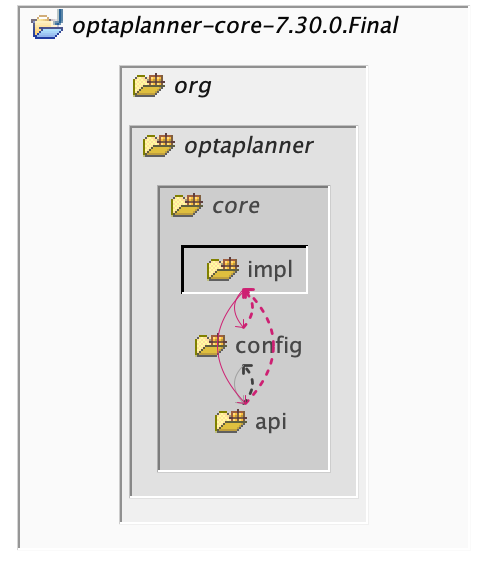
\includegraphics[width=0.4\textwidth]{figures/step2/allcomp.png}}
    \hfill
    \centering
    \subfloat[\label{subfig:impl-src}A more detailed dependency graph between the Configuration system and the Implementation system. Downward flow is depicted by full arrows, whereas upward flow is depicted with dotted-arrows. In this case, the upward flow shows which entities of the Configuration system \textit{are dependent on} the Implementation system. The vice-versa holds true for the downward flow.]{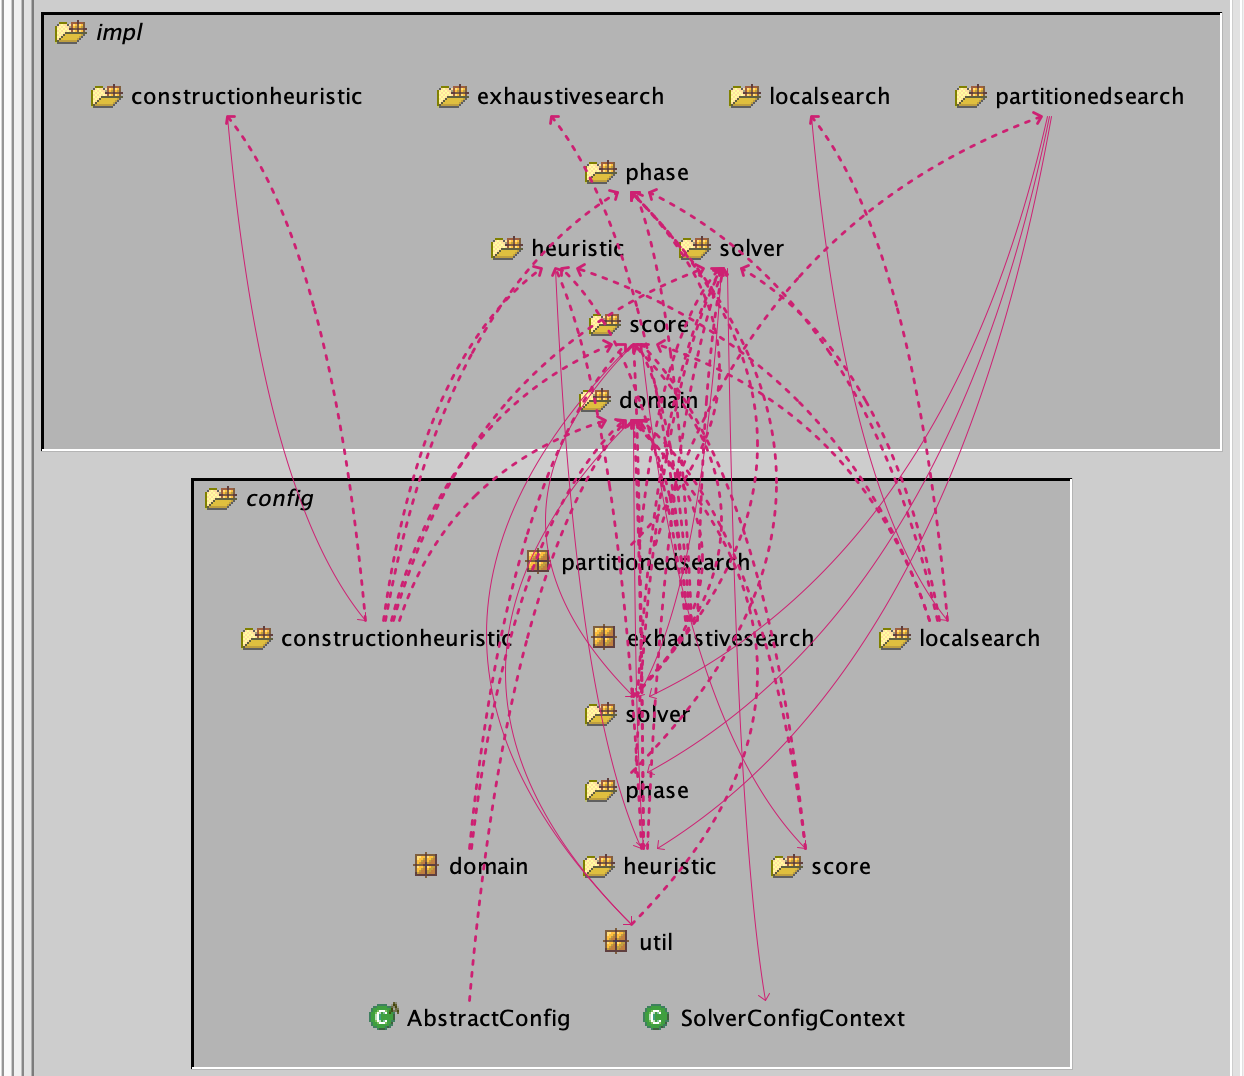
\includegraphics[width=0.48\textwidth]{figures/step2/impl-config.png}}
    % \caption{overall caption}
    % \label{}
\end{figure}
\subsubsection{Key information about the system}
\label{subsub:keyinfo}
Before we delve into further details about each one of the main architectural components of the system, we would like to establish some general information that will be useful for the following sections. There are two key concepts to this software whose definition should be tackled: the \textit{Solver} and the \textit{Solution}.
\paragraph{{\scriptsize SOLVER}}
\label{para:solver}
Is responsible for rendering one or more solutions to a given problem. The user has to provide information about what is expected of the solver via \verb!xml! files. For example, which optimization algorithms should be used. The Configuration system is mainly responsible for establishing the solver details and implementation.
\paragraph{{\scriptsize SOLUTION}}
Is the output that the user expects of OptaPlanner. The solution is defined as a separate class by the user and this class represents both, the \textit{definition} of the problem as well as its \textit{solution}, once it has been found. Therefore, when we refer to the problem, ultimately we also refer to its feasible solutions - perhaps a better naming convention is required. The OptaPlanner development team uses a generic class for defining this entity in the source code, namely \verb!Solution_!. The annotation for this class is \verb!@PlanningSolution!. Using annotations eliminates the need for declaring classes/objects because the system can find them automatically via the classpaths defined in the \verb!xml! files.\\\\
We would also like to emphasise the following \textbf{facts}:
\begin{enumerate}[label=(\roman*)]
    \item Each \textit{solver} can only solve one problem at a time.
    \item Each problem can have none, one, or more than one solution because the user can decide whether he wants to run none, one or multiple optimization algorithms.
    \item Every running instance of the problem - in order to find a solution - is called a \underline{Phase}. Since the problem can run multiple times via the multiple algorithms, the problem can also have multiple \textit{phases}.
    \item Determining the fitness of each solution is also established by the user in the \verb!xml! files, and therefore, decoded by the Configuration system.
\end{enumerate}
\subsubsection{Other entities of the architecture}
\label{sec:arch_entities}
There are several other entities that are present in the architecture of the system which represent some key concepts with regard to how OptaPlanner is developed. Moreover, the implementation of these entities is encompassed in more than one architectural component. Therefore, in order to keep this document as compact as possible, we first give an introduction of these key concepts and explain why they are relevant to OptaPlanner.
\paragraph{{\scriptsize DOMAIN}}
The domain modules are relevant to the system because they help define the key facts of every problem. In our model, the domain would contain objects such as Queens, column, rows, points. Defining a proper domain is essential to establishing a problem and its solution. This entity is present in all three architectural components.
\paragraph{{\scriptsize SCORE}}
The score is used to define `how good’ a \textit{solution} is, and it is a crucial aspect to OptaPlanner because it is the most objective way that solutions can be compared to one another, before establishing the best one that the system will return. Similarly to the previous entity, \textit{score} is also present in all three architectural components.
\paragraph{{\scriptsize PHASE}}
The \textit{phase} represents a running instance of an algorithm solving a given problem. It is a relevant concept to OptaPlanner because the user can decide to have multiple optimization algorithms run with the same problem and as such, it is important for all the results to be defined and saved. The \textit{phase} entity makes this possible. This entity is present in the Configuration and Implementation systems.
\paragraph{{\scriptsize CONSTRUCTION HEURISTICS}}
This entity is developed so that it can produce an initial \textit{solution} to the input problem in a finite amount of time. The solution does not necessarily need to be feasible, but this is usually not an issue because one of the optimization algorithms is almost always used for solving the problem. However, some of these algorithms need to make use of this entity which is why the \textit{Construction Heuristics} is relevant for the system. The entity is present in the Configuration and Implementation systems.
\paragraph{{\scriptsize THE ALGORITHMS}}
\label{par:algos}
The optimization algorithms are relevant to the software because they provide possible (and optimal) solutions for the input problems. The OptaPlanner team has implemented three algorithms: exhaustive search, local search and partitioned search. Exhaustive search is not very efficient because it always looks for the global optimum. Therefore, it can be very hard to scale with it. The local search algorithm uses a single-search path and moves facts around to find a good feasible solution. However, it needs to start with an initialized solution, which is why it required to make use of the \textit{Construction Heuristics}. Partitioned search is a more efficient algorithm because the data set is partitioned into several parts which can be worked on simultaneously by multiple threads. The results are nearly optimal.
\subsubsection{The concept of Scope in OptaPlanner}
We provide an explanation for the concept of \textit{scope} in this system because it is relevant to our analysis, the complexity of the system and its main functionalities. 
The \textit{scope} can have multiple definitions in OptaPlanner. First, there is the scope of the \underline{solver}, the outermost scope. Then, there is the scope of the \underline{phase}. The end of a phase depicts the start of another one, and therefore, the start of another phase scope. 
Every phase (also known as optimization algorithm) has \underline{steps}. In our example model of the NQueens a step is defined as a general displacement of a queen. Every step, can also have \underline{moves}. In our example algorithm, a move is entitled to displacing a queen either by one position horizontally or vertically. Therefore, the phase scope encapsulates the step scope, which can also encapsulate the move scope. The move scope is possibly the innermost scope level.
Figure \ref{fig:scope_fig} depicts the definition of scope for our example model, the NQueen problem.
\label{subsub:scope}
\begin{figure}[H]
    \centering
    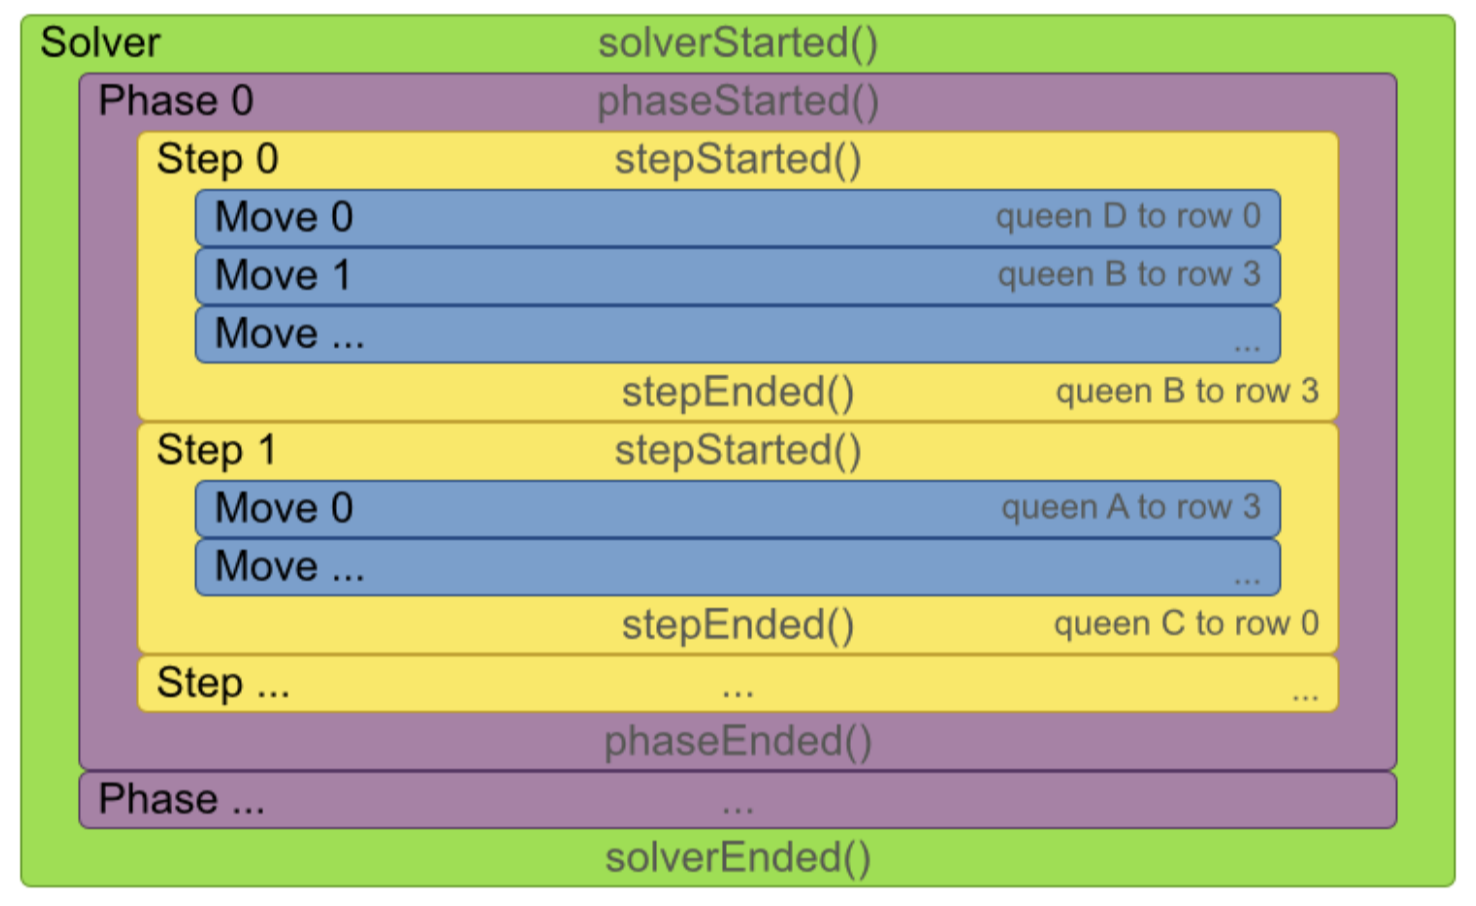
\includegraphics[width=0.48\textwidth]{figures/step2/scope_overview.png}
    \caption{Scope}
    \label{fig:scope_fig}
\end{figure}